% Project Specifications
\clearpage%if the chapter heading starts close to bottom of the page, force a line break and remove the vertical vspace
\vspace{21.5pt}
\chapter{Implementation}
\section{Software  setup}

First state of project was getting initial programming environment ready, consisting of rp2040 SDK, Arm GCC cross compiler and visual studio code with plugins for debugging and managing the rp2040 CMAKE build process, and a j-link SWD debugger to program and debug on the \gls{mcu} more flexibly than \gls{usb} UF2 flash programming. A logic analyser was also used in initial phases to help monitor the debug traffic for verification of handshake operations till communication was established between boards.
\clearpage
\section{Hardware setup}
%
\begin{figure}[ht]
	\centering
	\AltText{Initial POC hardware setup showing direct soldered wiring between J-Link Edu and a Raspberry pi Pico}{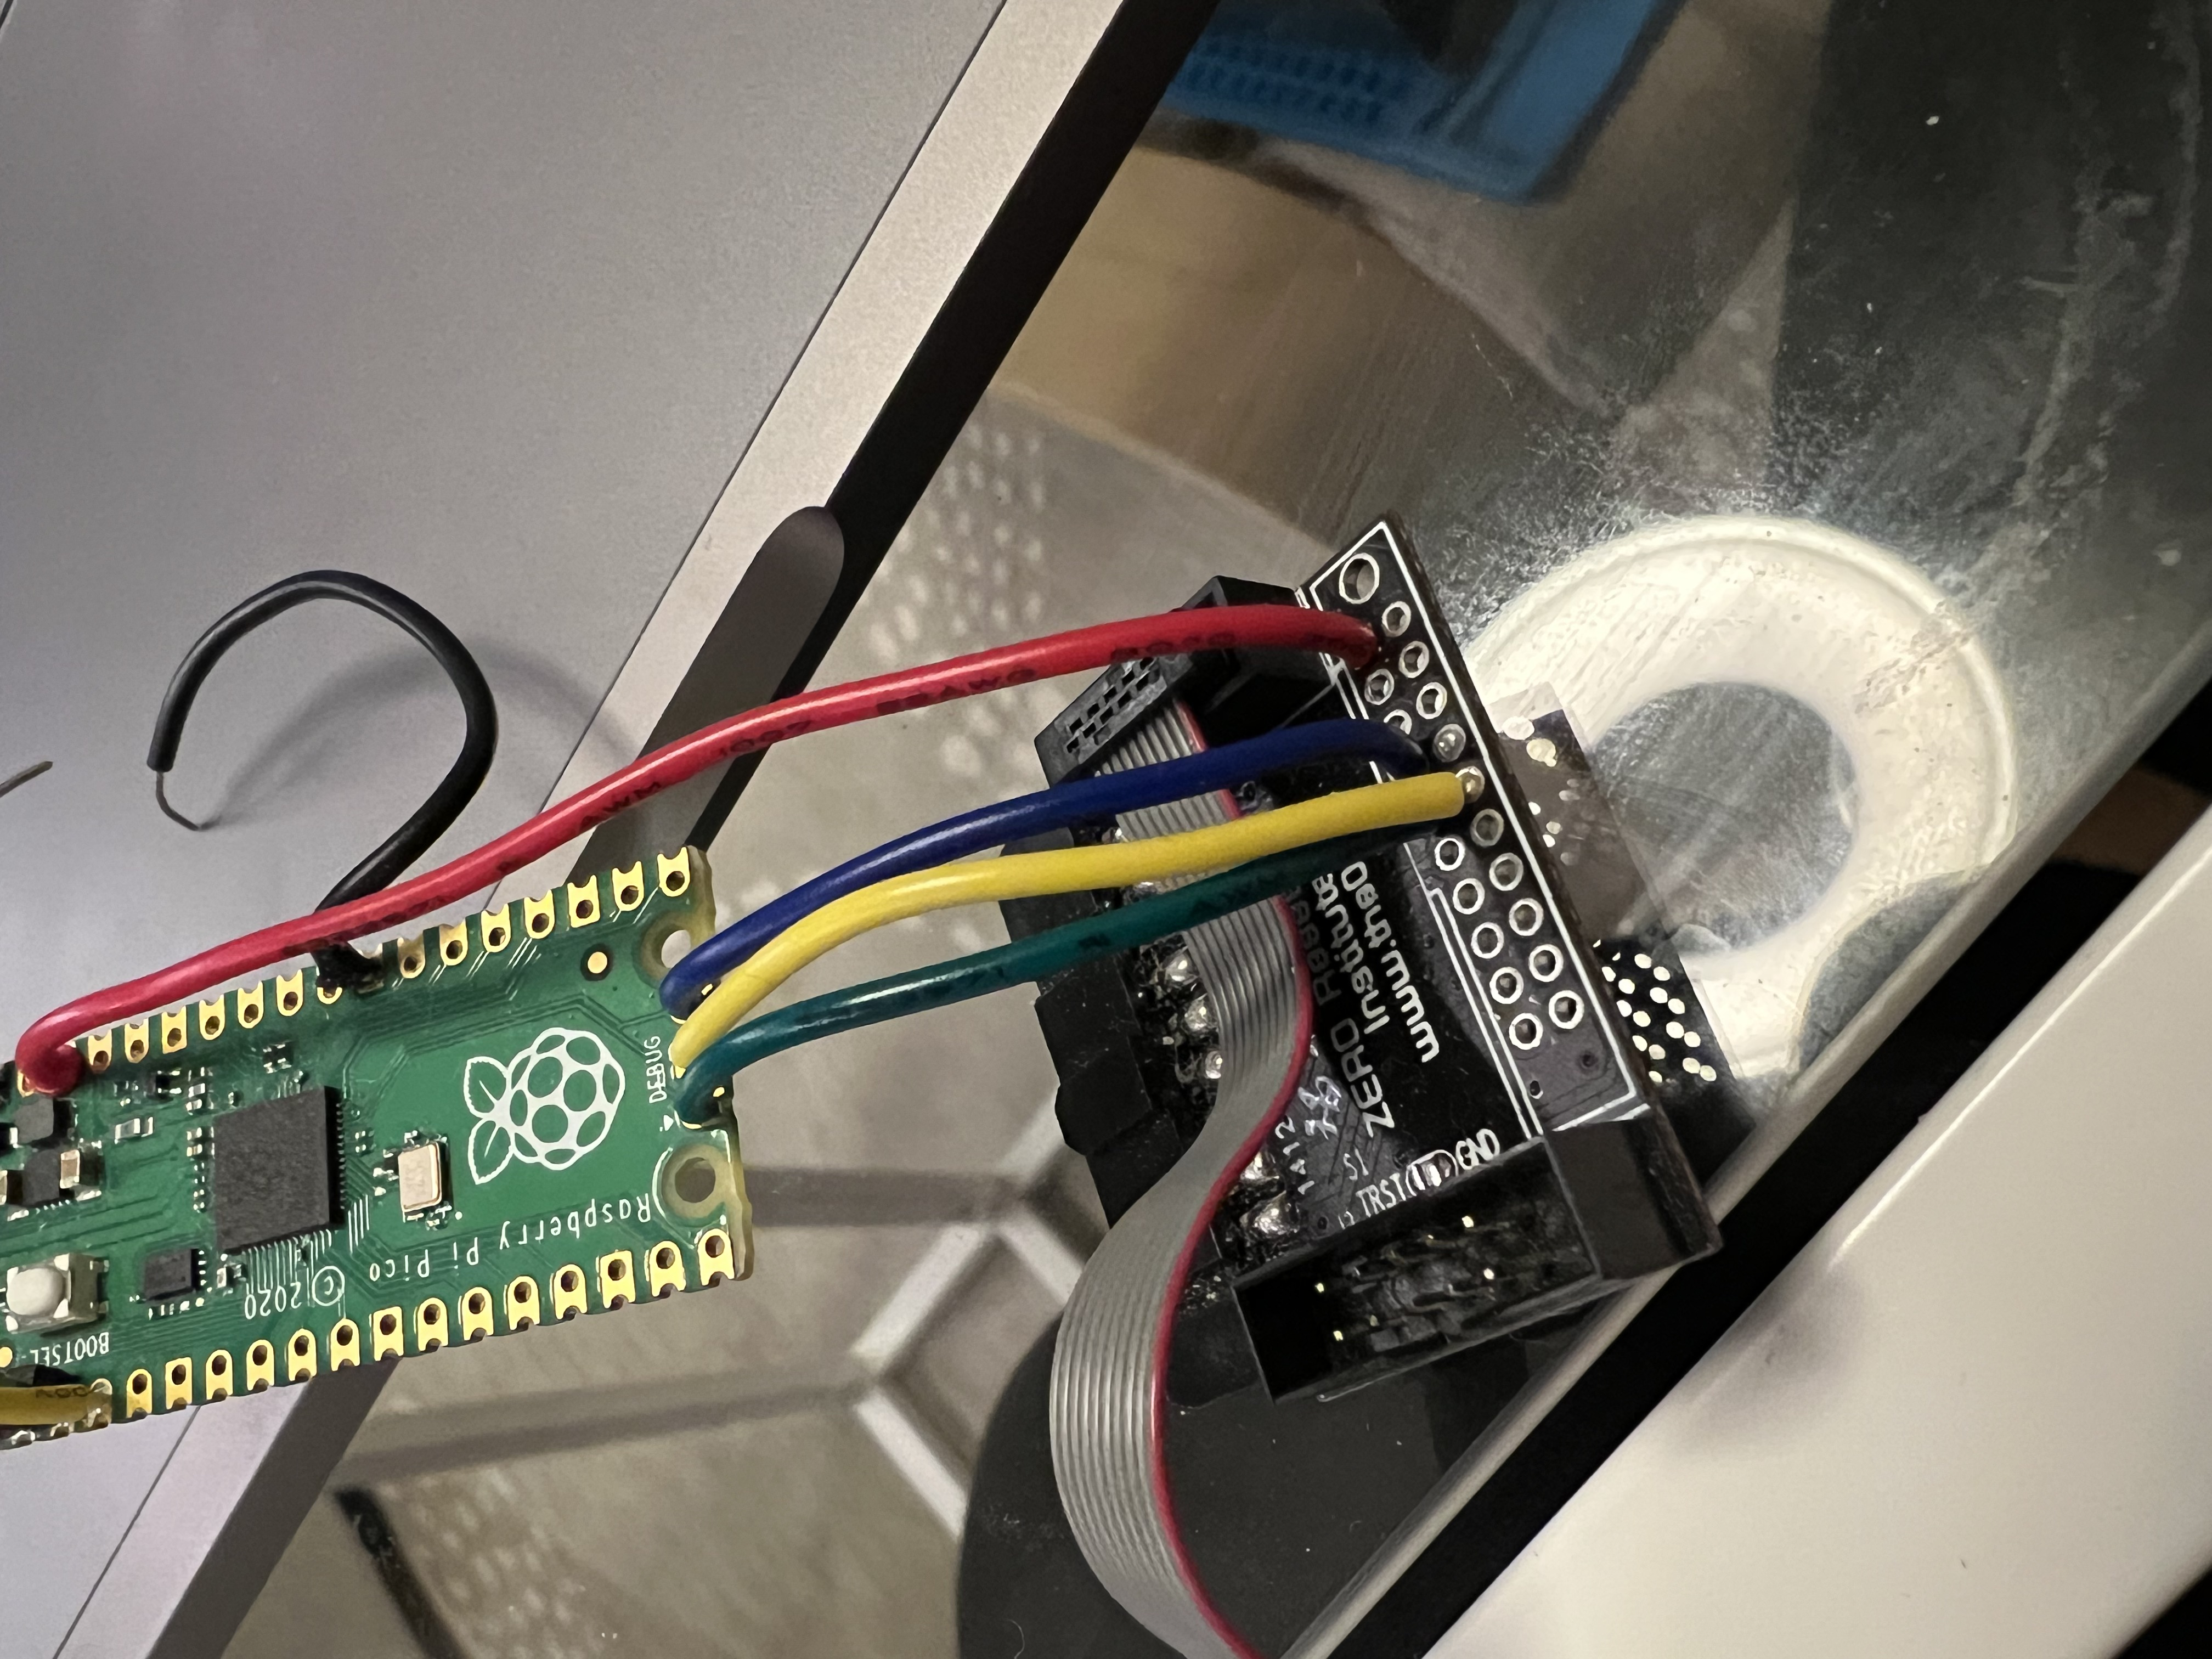
\includegraphics[width=\textwidth]{initial POC setup}}
	\caption{initial POC setup}
	\label{fig:InitialPOCwiring}
\end{figure}

For current proof of concept test bench setup a pair of Pi Pico was directly wired into a J-Link debugger with directly soldered wires for simplicity as show in \autoref{fig:InitialPOCwiring}.

Segger RTT is used for debug console access during testing to eliminate need for a seperate UART/Serial receiver and associated wiring.

In the final test setup a jumper cable is used to simulate the closing of a mounting interface interlock to similate plugging and unplugging target board without physically removing jumper wires from bench setup.

%\pagebreak
\begin{figure}[ht]
	\centering
	\AltText{Full POC hardware setup showing display and buttons for UI on breadboads along with target device}{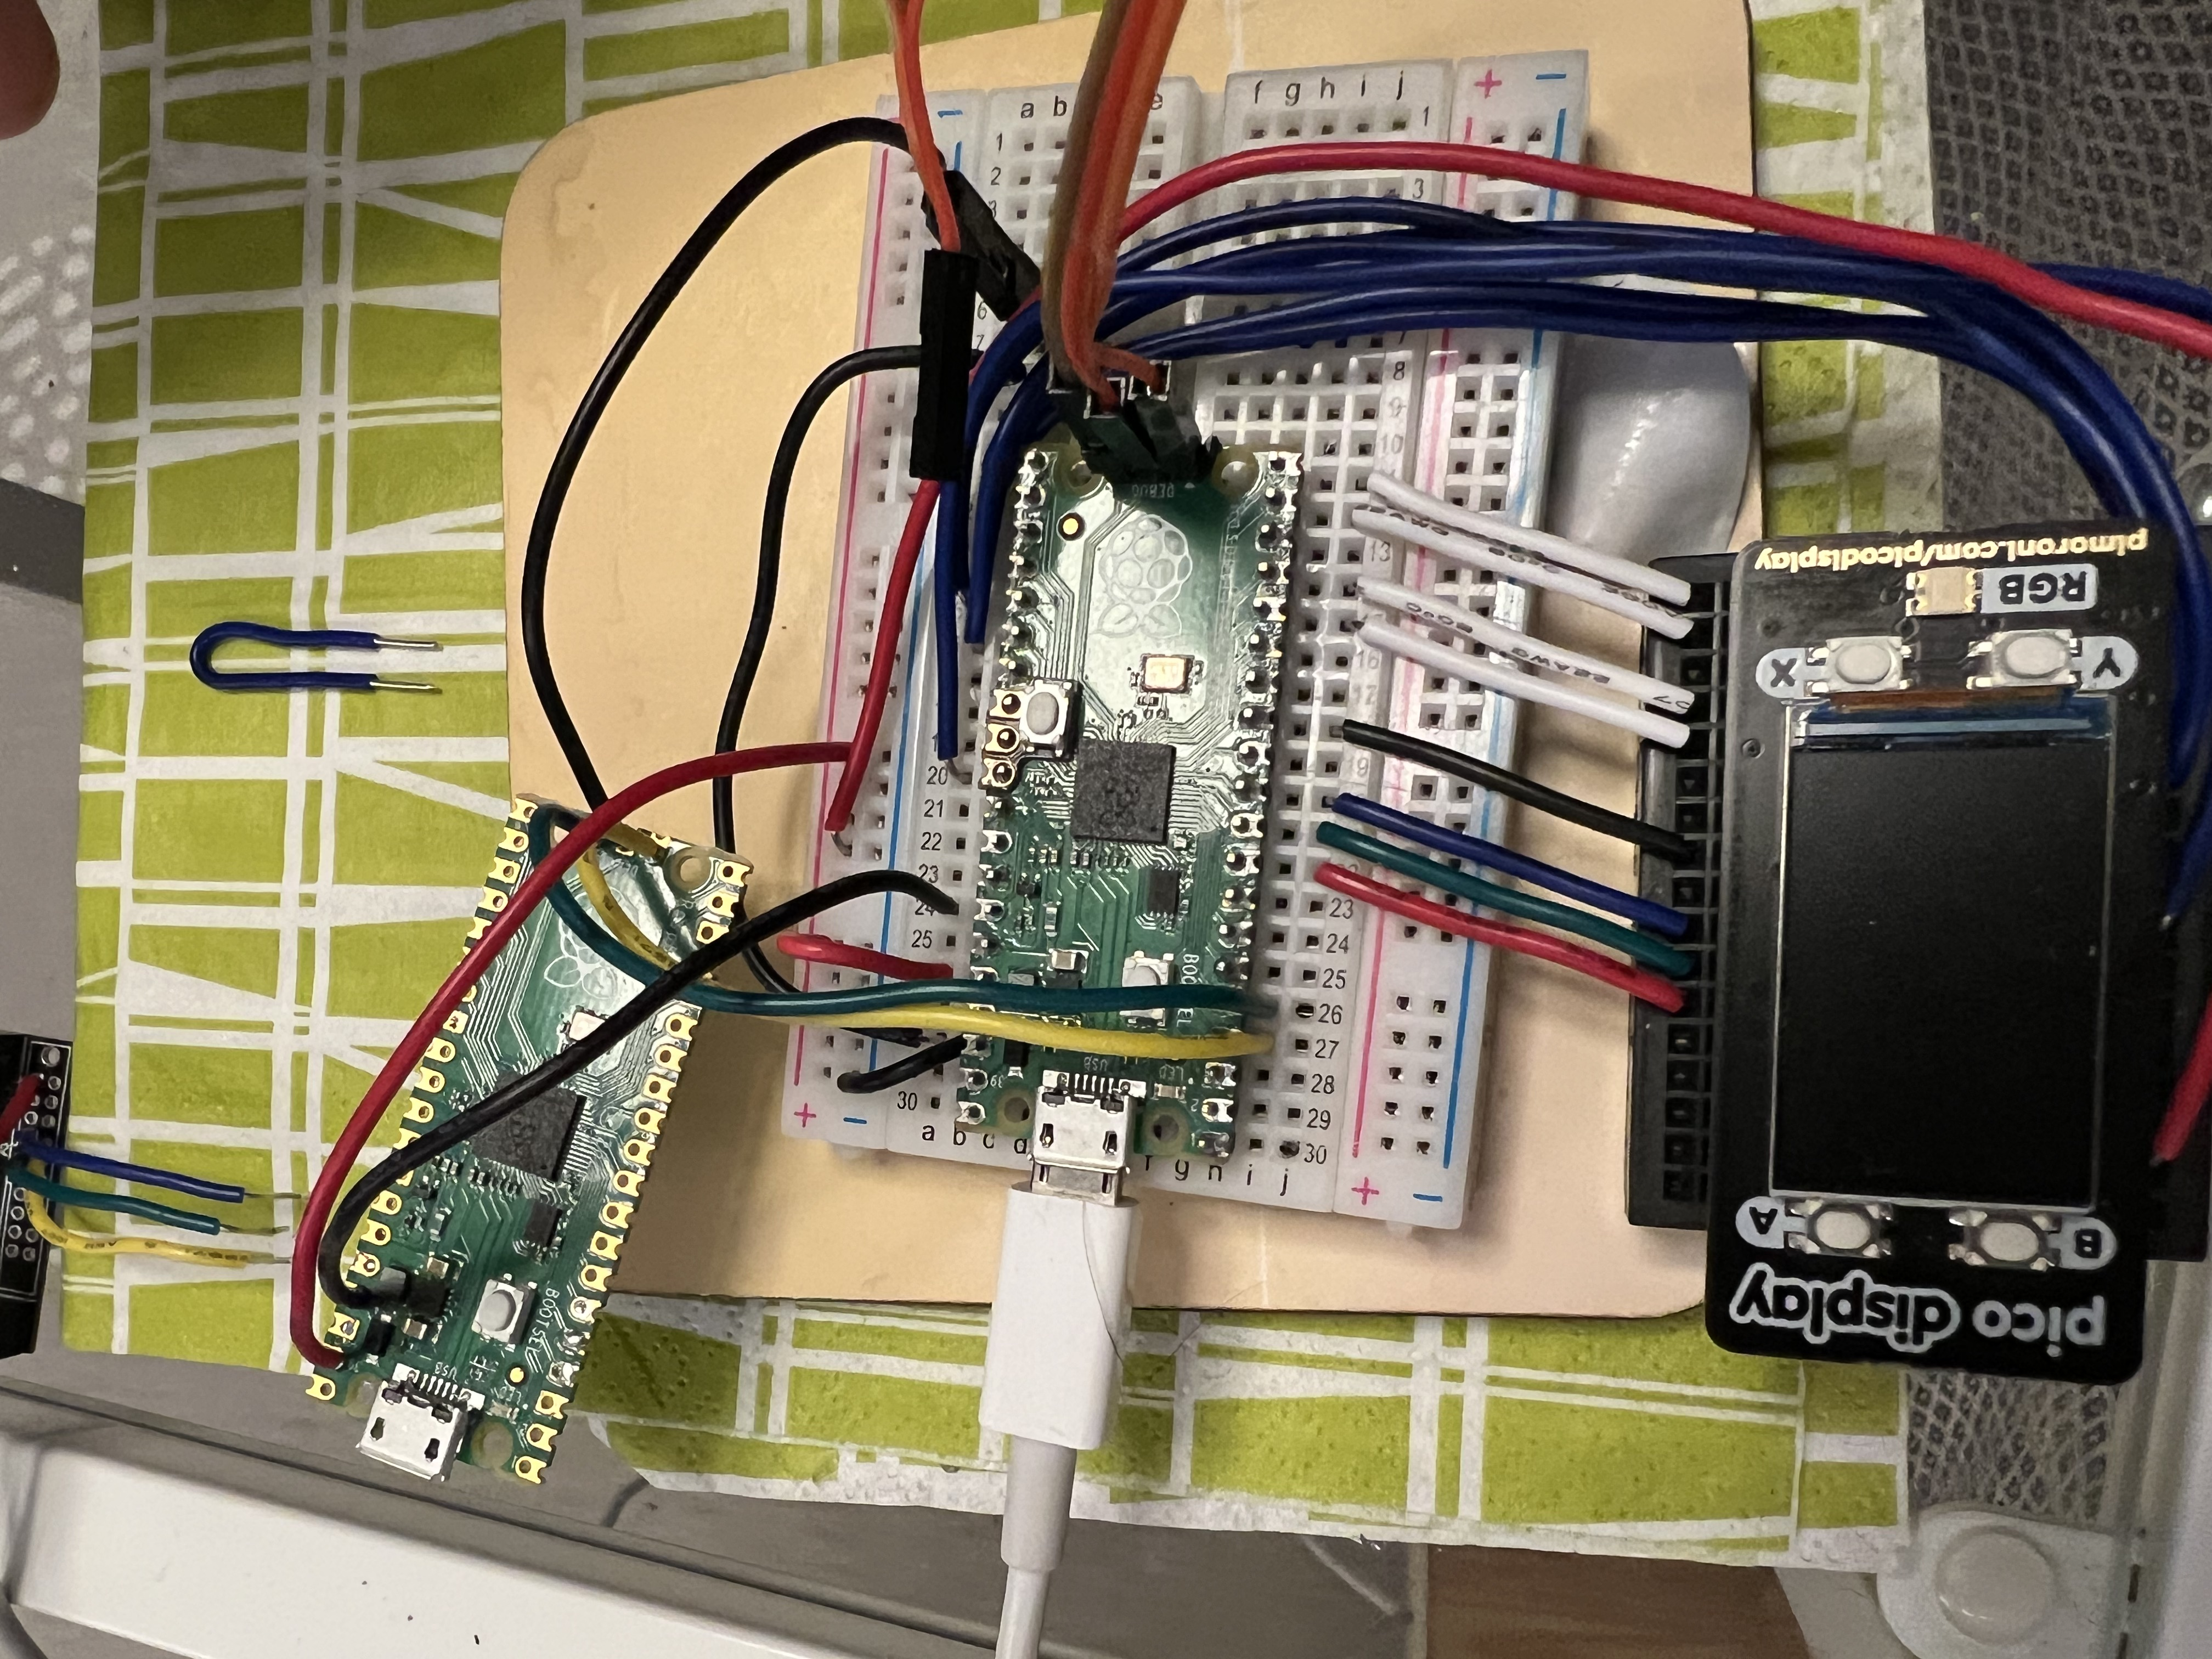
\includegraphics[width=\textwidth]{full POC setup}}
	\caption{Full wiring on breadboard with Interface}
	\label{fig:FullPOCwiring}
\end{figure}

This was later expanded to include a Pimoroni display and buttons for a user interface, and second Pi Pico as flashing target \autoref{fig:FullPOCwiring}.

\clearpage
\section{Software bootstrap}
Initial step was to establish \gls{swd} setup as lowest level critical component, this took longer than anticipated after initial response reading DPIDR register succeeded to verify an \gls{arm} debug unit was responding, but further attempted operations such as memory read failed. Reason for failure transpired to a lack of accounting multiple debug units\cite{raspberrypiltdRaspberryPiPico} with many references to \gls{swd} implementation omitting the step of device selection from the setup sequence owing to most \gls{arm} \gls{mcu}'s only having one core this being an uncessary step.

Once handshake was established the most critical functions of memory write and read were implemented and verified to confirm successful control over \gls{swd}, 

From there a small \gls{ram} resident test program to blink the onboard \gls{led} was created as a test case binary to to be write and executed from memory via \gls{swd} for a simple control verification, initially merely blinking \gls{led} to confirm code execution before building a shared memory structure for executing commands such as file recovery or flash programming/erasing.

This uses magic numbers and checksums for validation, and writing result codes back to memory that can be read by recovery device.

Programming sequence example to bootstrap running code on the target can be found in Appendix 1.

It was determined that 'bit banging' the \gls{swd} bus was sufficiently performant to not need, the 40kB helper application only takes 51ms to send over the bus, and for flashing data the flashing process itself is so much slower than the data transfer that the \gls{swd} speed becomes a non issue.


interleave loading of fw data sent ok took 4154ms
without interleave data sent ok took 5562ms

20\%+ flash speed increase for using interleave, simple optimisation


Picture of loading UI

Picture of flashing operation


\clearpage
\section{File system implementation}

Due to the large amounts of repeated information and empty space within a UF2 format file direct storage into the pico's flash was impractical, especially with the effective requirement to store separate images for standard pico and W variations, which added together can reach a size bigger than the whole flash storage.

To enable maximum practical storage a more compact storage solution was implemented, consisting of three data areas for the UF2 image.

Laid out as follows: Data area, consisting of all the 256byte data packets from each UF2 block, An address area, indexing each of these data packets to their destination address and finally a header block where the filename, and other related metadata such as block count are stored. UF2 block /gls{crc} values were not stored and recalculated at runtime. Though a single checksum of all the data should still be added for verification before start of flashing.

Due to the requirement to store two images, there are two of these data structures kept, with the W one allocated the bulk of the storage to allow for the wireless module firmware and drivers taking up notably more storage than the regular pico as presented in table \ref{table:file_storage}:


\begin{table}[h]
	\centering
	\caption{Flash Storage layout}%IMPORTANT the caption must be before the tabular, so it will be on top of the table (there are other tricks to force it on top; but this one is straightforward).
	\vspace{-16.5pt}%time to time, spacing between caption and table can go too big...

		\begin{tabular}{|l|l|l|}
			\hline
			Address & Size  & Contents        \\ \hline
			0x000000 & 256kB & Program + Helper binary \\ \hline
			0x040000 & 4kB & UF2 Header 1      \\ \hline
			0x043000 & 12kB & UF2 Addresses 1 \\ \hline
			0x044000 & 600kB & UF2 Data 1 \\ \hline
			0x0D9000 & 4kB & UF2 Header 1 \\ \hline
			0x0DA000 & 20kB & UF2 Addresses 2      \\ \hline
			0x0DE000 & 1152kB & UF2 Data 2 \\ \hline
			0x1FFFFF & & End of flash. \\ \hline
		\end{tabular}
		\label{table:file_storage}
\end{table}

The \gls{usb} Virtual File System presented for UF2 image storage is based upon the TinyUF2 bootloader\cite{TinyUF2Bootloader2023}, which has been repurposed to capture file system uf2 transfer and store it to the internal UF2 storage.

To keep the files consistent even if power loss were to happen the file data is cleared at start of transaction, and header only written back once the full data is stored. Thus a power loss or other unexpected event mid transfer will leave the board with an empty file slot instead of inconsistent data.

One of the notable changes made to the TinyUF2 bootloader is to capture the file system information more fully, in order to read and store the full long file name of the UF2 image so that this can be presented to the user as an aid memoir on what firmware is loaded. This filename is also dynamically written to the virtual file system upon USB connection to present the data there also.

This required cacheing more of the \gls{fat} table than previously needed, due to long file names potentially requiring more than first cluster, especially with operating systems such as macOS that can also write other hidden helper files to the file system that need to be ignored.

Another modification over TinyUF2 loader is for the virtual image to present the currently stored image on the presented file system in recreated form when \gls{usb} loading is active including the current stored image size instead of presenting full flash image as originally designed, allowing end user to retrieve the image back off device as well as replace the stored image with an updated one.

\clearpage
\section{Testing}

For testing functionality, various likely scenarios were setup and verified to be repeatable.

First tests consisted of setting up recovery scenarios on MicroPython via Thonny\cite{ThonnyPythonIDE}, creating startup python scripts that both block the USB port or just run, and performing a recovery procedure to verify that the file is renamed successfully, or deleted, if a previous recovery result is still present.

Second tests verified that a populated file system could be wiped on an existing MicroPython install.

Third tests verified loading of different uf2 firmware files to the recovery platform, and then reflashing a target pico with the loaded firmware.



